\documentclass{article}

%\usepackage{mathtools}
\usepackage{amsfonts}
\usepackage[spanish,mexico]{babel}
\usepackage[utf8]{inputenc}
\usepackage{graphicx}
\usepackage{subcaption}
\usepackage{booktabs}
\usepackage{url}
\usepackage{listings}%http://www.tex.ac.uk/FAQ-codelist.html
\usepackage{color}

\definecolor{codegreen}{rgb}{0,0.6,0}
\definecolor{codegray}{rgb}{0.5,0.5,0.5}
\definecolor{codepurple}{rgb}{0.58,0,0.82}
\definecolor{backcolour}{rgb}{0.95,0.95,0.92}

\lstdefinestyle{mystyle}{
  backgroundcolor=\color{backcolour},
  commentstyle=\color{codegreen},
  keywordstyle=\color{magenta},
  numberstyle=\tiny\color{codegray},
  stringstyle=\color{codepurple},
  basicstyle=\footnotesize,
  breakatwhitespace=false,
  breaklines=true,
  captionpos=b,
  keepspaces=true,
  numbers=left,
  numbersep=5pt,
  showspaces=false,
  showstringspaces=false,
  showtabs=false,
  tabsize=2
}

\lstset{style=mystyle}
\graphicspath{ {img/} }
%\usepackage{enumitem}
%\usepackage{tikz}

\title{Grafos en red, distancia Manhattan y percolación de vecindades}
\author{José Alberto Benavides Vázquez}
\date{\today}

\begin{document}

  \maketitle

  \section{Introducción}

  Esta práctica se realizó a partir de un programa en desarrollo para flujo en redes alojado en \url{https://github.com/jbenavidesv87/FlujoRedes}. El código de esta práctica puede consultarse en \url{https://github.com/jbenavidesv87/FlujoRedes/tree/master/ejemplos/08Rejilla} \cite{Grafos}.

  En esta simulación se generan grafos con $k \times k, k = \{ 3, 4, 5, 6, 7, 8, 9, 10 \}$ nodos dispuestos en forma de red, conectados con vecinos a una distancia Manhattan $l = \{ 1, 2, 3 \}$ y con con una probabilidad $p = \{ 0, 0.02, 0.04, 0.06, 0.08, 0.1 \} $ de conectarse de manera aleatoria con otro nodo elegido al azar entre los nodos disponibles que no formen parte de su vecindad, todo esto con el fin de estudiar el comportamiento del flujo máximo entre un nodo inicial y uno final ocasionado por la percolación de aristas en grafos así definidos.


  \section{Descripción de la implementación del modelo}

  La disposición de grafos en forma de red se logró mediante la implementación del método \texttt{Cuadrado} a la clase \texttt{Grafo} del programa inicialmente mencionado:

  \begin{lstlisting}[language = Python]
def Cuadrado(self, nodos):
  N = len(nodos)
  lado = floor(sqrt(N))
  for i in range(N):
    n = nodos[i]
    n.radio = 1 / N
    n.posicion = ((i % lado) / (lado - 1), 1 - int(i / lado) / (lado - 1))
  \end{lstlisting}

  Esta función obtiene la longitud de una lista de nodos (línea $2$), calcula el piso de la raíz cuadrada para obtener cuántos nodos ha de haber por lado (línea $3$) y cada nodo de la lista se sitúa en una posición dada por esa cantidad de nodos por lado (línea $7$).

  Las conexiones en Manhattan se realizaron por el método \texttt{PasoManhattan} integrado a la clase \texttt{Grafo}:

  \begin{lstlisting}[language = Python]
def PasoManhattan(self, n, v, paso, nuevasVecindades = None):
  if self.dirigido:
    for  v1 in self.vecinos[v]:
      self.ConectarNodos(n, v1)
      if paso > 1:
        self.PasoManhattan(n, v1, paso - 1)
  else:
    for v1 in self.vecinos[v]:
      if n != v1:
        nuevasVecindades.append((n, v1))
      if paso > 1:
        self.PasoManhattan(n, v1, paso - 1, nuevasVecindades)
    return nuevasVecindades

for i in range(k - 1):
  if i % lado != lado - 1:
    G.ConectarNodos(G.nodos[i], G.nodos[i + 1])

  if int(i / lado) < lado and i < lado ** 2 - lado:
    G.ConectarNodos(G.nodos[i], G.nodos[i + lado])

a = [] # Nuevas vecindades
  for n in G.nodos:
    for v in G.vecinos[n]:
      a = G.PasoManhattan(n, v, l - 1, a)
  for par in a:
    G.ConectarNodos(par[0], par[1])
  \end{lstlisting}

  Este método da por cada nodo $l$ pasos en Manhattan. Cada paso que da implica una conexión con un vecino, luego, de manera recursiva, los nodos siguientes dan $l - 1$ pasos y se conectan con los nodos adyacentes a esa distancia Manhattan.

  Los grafos resultantes para estos parámetros y con estas especificaciones se graficaron y se almacenaron en una animación \texttt{gif} que puede consultarse en \url{FALTA}. Asímismo, se muestran ejemplos de estos grafos en la figura \ref{ejemplosGrafos} (p. \pageref{ejemplosGrafos}).

  \begin{figure}[h] %https://tex.stackexchange.com/questions/167770/forcing-figure-with-4-subfigures-to-span-over-twocolumns
    \centering
    \begin{subfigure}[b]{0.45\textwidth}
      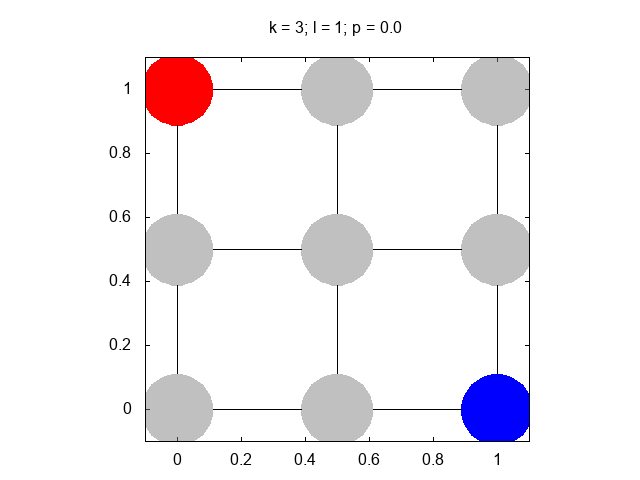
\includegraphics[width=\textwidth]{k009l001p000}
      \caption{Grafo con $9$ nodos y $l = 1$ vecindades en distancia Manhattan.}
      \label{fig:a}
    \end{subfigure}
    % this comment avoids break-line...
    \begin{subfigure}[b]{0.45\textwidth}
      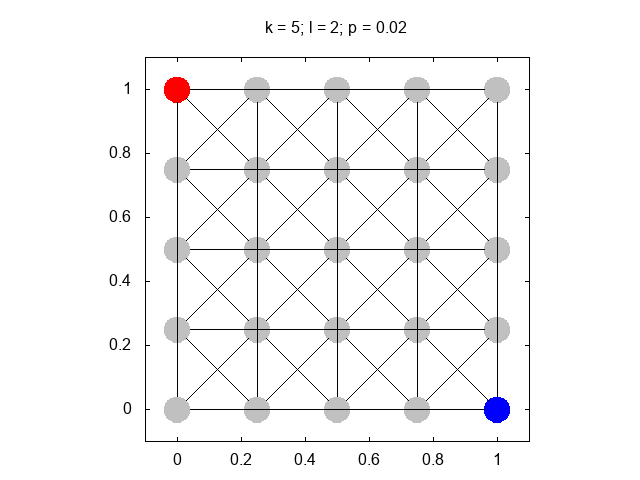
\includegraphics[width=\textwidth]{k025l002p020}
      \caption{Grafo con $25$ nodos y $l = 2$ vecindades en distancia Manhattan.}
      \label{fig:b}
    \end{subfigure}

    \begin{subfigure}[b]{0.45\textwidth}
      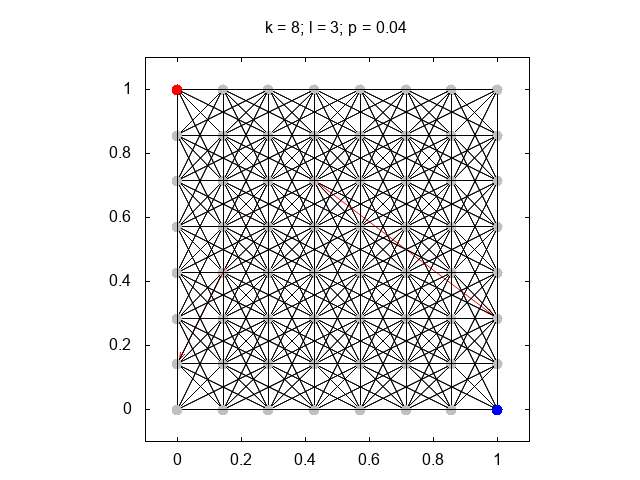
\includegraphics[width=\textwidth]{k064l003p040}
      \caption{Grafo con $64$ nodos y $l = 3$ vecindades en distancia Manhattan.}
      \label{fig:c}
    \end{subfigure}
    % ... this comment too
    \begin{subfigure}[b]{0.45\textwidth}
      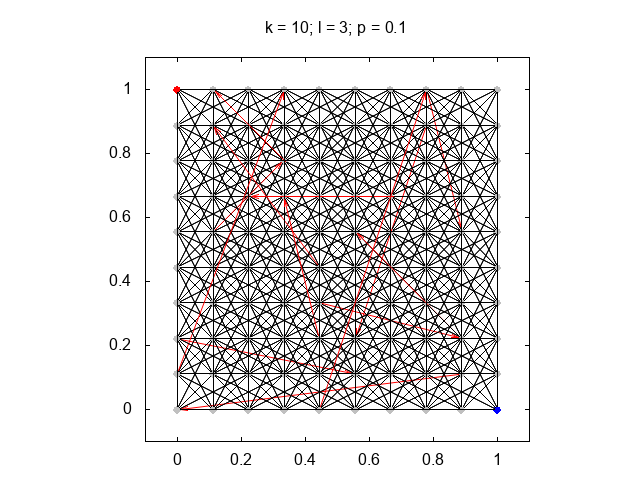
\includegraphics[width=\textwidth]{k100l003p100}
      \caption{Grafo con $100$ nodos y $l = 3$ vecindades en distancia Manhattan.}
          \label{fig:d}
    \end{subfigure}
    \caption{Ejemplos de grafos en red generados a partir de parámetros $k, l, p$ donde los nodos inicial y final aparecen en la esquina superior izquierda en azul y en la esquina inferior derecha en rojo respectivamente.}\label{ejemplosGrafos}
\end{figure}

  \section{Implementación del código de percolación de aristas}

  El código de percolación de aristas consiste en una función que elimina arcos de manera aleatoria en los nodos creados de la manera descrita en la sección anterior. Para eliminar estas aristas es necesario eliminar de la clase \texttt{Grafo} las vecindades y pesos que se establecen de manera predeterminada al conectar nodos entre sí. Este proceso se repite mientras haya caminos que lleven flujo del nodo inicial al final. Tal procedimiento se codificó en las siguientes líneas:

  \begin{lstlisting}[language = Python]
llega = True
  a = 0 # Cantidad de arcos eliminados
  while llega:
    tiempo = clock()
    ford = G.Ford_Fulkerson(G.nodos[0], G.nodos[k - 1])
    tiempo = clock() - tiempo
    if ford == 0:
      llega = False

    n = sample(set(G.nodos), 1)[0]
    candidatos = set(G.vecinos[n])
    if len(candidatos) > 0:
      v = sample(set(G.vecinos[n]), 1)[0]
      if v:
        del(G.pesos[(n, v)])
        G.vecinos[n].remove(v)
        if n in G.vecinos[v]:
          del(G.pesos[(v, n)])
          G.vecinos[v].remove(n)
        a = a + 1
  \end{lstlisting}

  \section{Ford--Fulkerson}

  Se midió el flujo máximo entre el nodo inicial y el final de cada grafo generado con base en los parámetros destritos en este reporte, los resultados se graficaron para cada $k, l, p$ en diagramas ternarios en los que se tomaron como ejes la probabilidad de establecer vecindades al azar $p$, el flujo máximo entre el nodo inicial y el final $f$ y la cantidad de arcos eliminados $a$. Una muestra de los diagramas ternarios generados se muestra en la figura \ref{tern} (p. \pageref{tern}). Una animación de la secuencia de estos diagramas puede consultarse en \url{FALTA}.

  \begin{figure}[h] %https://tex.stackexchange.com/questions/167770/forcing-figure-with-4-subfigures-to-span-over-twocolumns
    \centering
    \begin{subfigure}[b]{0.45\textwidth}
      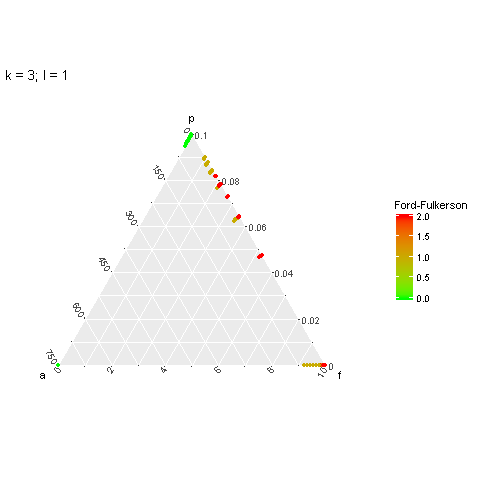
\includegraphics[width=\textwidth]{k009l001}
      \caption{Diagrama con $k = 3, l = 1$.}
      \label{fig:a}
    \end{subfigure}
    % this comment avoids break-line...
    \begin{subfigure}[b]{0.45\textwidth}
      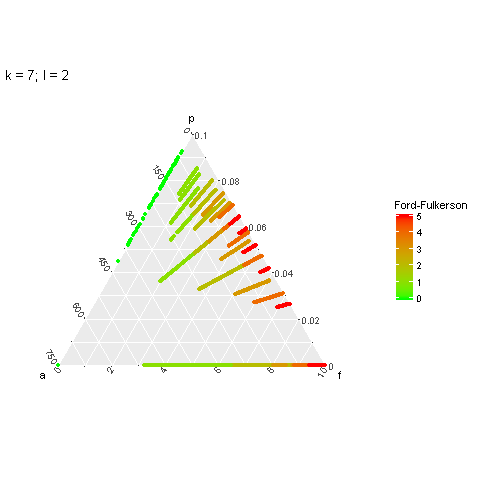
\includegraphics[width=\textwidth]{k049l002}
      \caption{Diagrama con $k = 7, l = 2$.}
      \label{fig:b}
    \end{subfigure}


    \begin{subfigure}[b]{1\textwidth}
      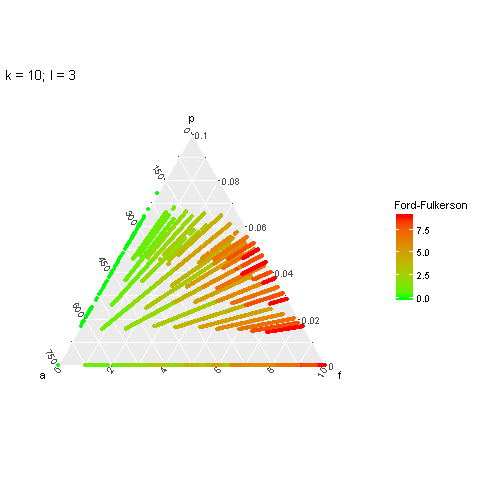
\includegraphics[width=\textwidth]{k100l003}
      \caption{Diagrama con $k = 10, l = 3$.}
          \label{fig:d}
    \end{subfigure}
    \caption{Ejemplos de diagramas ternarios donde se muestra la relación entre la probabilidad de establecer vecindades al azar $p$, el flujo máximo entre el nodo inicial y el final $f$, y la cantidad de arcos eliminados $a$.}\label{tern}
  \end{figure}

  Estas gráficas muestran que los flujos son máximos conforme aumenta la probabilidad $p$ de establecer vecindades al azar y se mantiene en el mínimo la cantidad $a$ de arcos eliminados, del mismo modo que aumentan cuando la distancia Manhattan para establecer vecindades aumenta también.

  Para valores por encima de los $64$ nodos con $l = 3$, la cantidad de arcos removidos debe ser al menos de un tercio del total de nodos para poner eliminar por completo el flujo entre el nodo incial y final de los grafos como los definidos en este reporte.

  \bibliography{biblio}{}
  \bibliographystyle{plain}

\end{document}
